\documentclass[answers]{exam}
\usepackage{marvosym}

%...TikZ & PGF
\usepackage{pgfplots}
\pgfplotsset{compat=1.11}
\tikzset{>=latex}
\usetikzlibrary{calc,math}
\usepackage{tikzsymbols}
\usepgfplotslibrary{fillbetween}
\usetikzlibrary{decorations.markings} 
\usetikzlibrary{arrows.meta} %...APP2 for arrows as objects and images
\usetikzlibrary{backgrounds} %...For shading portions of graphs
\usetikzlibrary{patterns} %...Unit 5 Problems
\usetikzlibrary{shapes.geometric} %...For drawing cylinders in Unit 2
\tikzset{
    mark position/.style args={#1(#2)}{
        postaction={
            decorate,
            decoration={
                markings,
                mark=at position #1 with \coordinate (#2);
            }
        }
    }
} %...See https://tex.stackexchange.com/questions/43960/define-node-at-relative-coordinates-of-draw-plot

\tikzset{
    declare function = {trajectoryequation10(\x,\vi,\thetai)= tan(\thetai)*\x - 10*\x^2/(2*(\vi*cos(\thetai))^2);},
    declare function = {trajectoryequation(\x,\vi,\thetai)= tan(\thetai)*\x - 9.8*\x^2/(2*(\vi*cos(\thetai))^2);},
    declare function = {patheq(\x,\yi,\vi,\thetai)= \yi + tan(\thetai)*\x - 9.8*\x^2/(2*(\vi*cos(\thetai))^2);},
    declare function = {patheqten(\x,\yi,\vi,\thetai)= \yi + tan(\thetai)*\x - 10*\x^2/(2*(\vi*cos(\thetai))^2);} %like patheq but with gravity = 10
}

%...siunitx
\usepackage{siunitx}
\DeclareSIUnit{\nothing}{\relax}
\def\mymu{\SI{}{\micro\nothing} }
\DeclareSIUnit\mmHg{mmHg}
\DeclareSIUnit{\mile}{mi}
%...NOTE: "The product symbol between the number and unit is set using the quantity-product option."

%...Other
\usepackage{amsthm}
\usepackage{amsmath}
\usepackage{amssymb}
\usepackage{cancel}
\usepackage{subcaption}
\usepackage{dashrule}
\usepackage{enumitem}
\usepackage{fontawesome}
\usepackage{multicol}
\usepackage{glossaries}
%\numberwithin{equation}{section}
\numberwithin{figure}{section}
\usepackage{float}
\usepackage{twemojis} %...twitter emojis
\usepackage{utfsym}
\newcommand{\R}{\mathbb{R}} %...real number symbol
\usepackage{graphicx}
\graphicspath{ {../Figures/} }
\usepackage{hyperref}
\hypersetup{colorlinks=true,
    linkcolor=blue,
    filecolor=magenta,
    urlcolor=cyan,}
\urlstyle{same}
\newcommand{\hdashline}{{\hdashrule{\textwidth}{0.5pt}{0.8mm}}}
\newcommand{\hgraydashline}{{\color{lightgray} \hdashrule{0.99\textwidth}{1pt}{0.8mm}}}

%...Miscellaneous user-defined symbols
\newcommand{\fnet}{F_{\text{net}}} %...For net force
\newcommand{\bvec}[1]{\vec{\mathbf{#1}}} %...bold vector
\newcommand{\bhat}[1]{\,\hat{\mathbf{#1}}} %...bold hat vector
\newcommand{\que}{\mathord{?}}  %...Question mark symbol in equation env
%...Define thick horizontal rule for examples:
\newcommand{\hhrule}{\hrule\hrule}
\let\oldtexttt\texttt% Store \texttt
\renewcommand{\texttt}[2][black]{\textcolor{#1}{\ttfamily #2}}% 

%...For use in the exam document class
\newif\ifprintmetasolutions


%...Decreases space above and below align and gather enironment
\makeatletter
\g@addto@macro\normalsize{%
  \setlength\abovedisplayskip{-3pt}
  \setlength\belowdisplayskip{6pt} 
}
\makeatother





\usepackage[margin=1in]{geometry}
\usepackage[figurewithin=none]{caption}
\usepackage{exam-randomizechoices}

\CorrectChoiceEmphasis{\color{red}\bfseries}
\renewcommand{\solutiontitle}{\noindent\textbf{\textcolor{red}{Solution:}}\enspace}

\usepackage{OutilsGeomTikz}
\usepackage{utfsym} %...Symbols in Unit 7 Problems
\usepackage{tabu} %...Symbols in Unit 7 Problems

%...For use in Unit 2            %    
\setlength{\columnsep}{2cm}      %
\setlength{\columnseprule}{1pt}  %
\usepackage[none]{hyphenat}      %
%%%%%%%%%%%%%%%%%%%%%%%%%%%%%%%%%

%...For use in Unit 11 on Waves:
\pgfdeclarehorizontalshading{visiblelight}{50bp}{  %
color(0.00000000000000bp)=(red);                   %
color(8.33333333333333bp)=(orange);                %
color(16.66666666666670bp)=(yellow);               %
color(25.00000000000000bp)=(green);                %
color(33.33333333333330bp)=(cyan);                 %
color(41.66666666666670bp)=(blue);                 %
color(50.00000000000000bp)=(violet)                %
}                                                  %

\newcommand{\checkbox}[1]{%
  \ifnum#1=1
    \makebox[0pt][l]{\raisebox{0.15ex}{\hspace{0.1em}\Large$\checkmark$}}%
  \fi
  $\square$%
}
%%%%%%%%%%%%%%%%%%%%%%%%%%%%%%%%%%%%%%%%%%%%%%%%%%%%

%...If using circuitikz package:
% \ctikzset{bipoles/battery1/height=0.5}
% \ctikzset{bipoles/battery1/width=0.25}
% \ctikzset{bipoles/resistor/height=0.15}
% \ctikzset{bipoles/resistor/width=0.4}

\newif\ifversionKlevel

%\versionKleveltrue
\versionKlevelfalse

\setrandomizerseed{1}
\bracketedpoints

\setlength{\columnsep}{2cm}
\setlength{\columnseprule}{1pt}
\usepackage[none]{hyphenat}

\firstpageheader{Physics L}{Unit 2: Force Interactions}{Test}
\runningheader{}{}{}

\ifversionKlevel
    \firstpageheader{Physics K}{Unit 2: Force Interactions}{Test}
    \runningheader{}{}{}
\fi

\begin{document}
\begin{questions}

% \question %...originally in unit 5: force analysis
% The free body diagram below represents the forces acting on the box in the image beside it. Given the scenario in the image, which force is missing from the free body diagram?

% \begin{center}
%     \begin{tikzpicture}
%         \node at (0,0) {\includegraphics[width=3cm]{z-other/L-physics/other/unit-6-projectile-motion/box.png}};
%         \begin{scope}[xshift=4cm]
%             \fill (0,0) circle (3pt);
%             \draw[<->] (-1,0) node[left] {?} -- (1,0) node[right] {$f$};
%             \draw[<->] (0,-1) node[below] {$F_g$} -- (0,1) node[above] {$F_N$};
%         \end{scope}
%     \end{tikzpicture}
% \end{center}

% \begin{randomizeoneparchoices}[norandomize]
%     \choice frictional force
%     \choice weight force
%     \correctchoice tension force
%     \choice normal force    
% \end{randomizeoneparchoices}

\question %...originally from unit 5: force analysis
A box slides across a smooth frictionless floor as shown in the image below.  What forces act on the box?

\begin{center}
    \begin{tikzpicture}
        \draw[fill=black!20] (0,0) rectangle (1,1) node[pos=0.5] {box};
        \draw[right=1cm,above=0.5cm,thick] (0,0) -- (3,0) node[above,pos=0.5] {rope};
        \draw[left=2cm] (0,0) -- (7,0);
    \end{tikzpicture}
\end{center}


\begin{randomizechoices}[norandomize]
    \choice tension, gravity
    \choice tension, gravity, normal force, friction
    \correctchoice tension, gravity, normal force
    \choice gravity, normal force, friction
\end{randomizechoices}

\question 
A baby elephant stands on the bed. Which of the following is a correct force pair?

\begin{center}
    \begin{tikzpicture}
        \node at (0,0) {\twemoji[width=3cm]{1f6cf}};
        \draw[above=4.2mm,right=-6mm] (0,0) node {\twemoji[height=1.7cm]{elephant}};
    \end{tikzpicture}
\end{center}

\begin{randomizechoices}[norandomize]
    \choice The force of the Earth on the bed ($F_\text{bed-earth}$), and the force of the elephant on the Earth ($F_\text{earth-elephant}$).
    \choice The force of the Earth on the bed ($F_\text{bed-earth}$), and the force of the elephant on the bed ($F_\text{bed-elephant}$).
    \correctchoice The force of the Earth on the bed ($F_\text{bed-earth}$), and the force of the bed on the Earth ($F_\text{earth-bed}$).
    \choice The force of the Earth on the elephant ($F_\text{elephant-earth}$), and the force of the bed on the elephant ($F_\text{elephant-bed}$).
    
\end{randomizechoices}


\question
The graph below shows the velocity of a car that is moving in a straight line.

\begin{center}
    \begin{tikzpicture}
        \begin{axis}[width=7cm,
            height=5cm,
            xmin=0,xmax=50,
            ymin=0,ymax=35,
            xlabel={Time (s)},
            ylabel={Velocity (m/s)},
            xtick={0,10,...,50},
            ytick={0,10,...,30},
            axis lines=left,
            grid=both,
            clip=false,
            minor tick num=1,
            ]
            \coordinate (q) at (0,0);
            \fill (q) circle (2pt);
            \node[above] at (3.5,0) {$q$};
            \coordinate (r) at (10,20);
            \fill (r) circle (2pt);
            \node at (r) [above=2pt] {$r$};
            \coordinate (s) at (20,20);
            \fill (s) circle (2pt);
            \node at (s) [above=2pt] {$s$};
            \coordinate (t) at (30,30);
            \fill (t) circle (2pt);
            \node at (t) [above=2pt] {$t$};
            \coordinate (u) at (40,10);
            \fill (u) circle (2pt);
            \node at (u) [right=2pt] {$u$};
            \draw[thick] (q) -- (r) -- (s) -- (t) -- (u);
        \end{axis}
    \end{tikzpicture}
\end{center}

During which of the following intervals are forces on the car balanced?

\begin{randomizeoneparchoices}[norandomize]
    \choice $q$ to $r$
    \correctchoice $r$ to $s$
    \choice $s$ to $t$
    \choice $t$ to $u$
\end{randomizeoneparchoices}

\question 
A paper is sitting at rest on your desk.  Which of the following statements best describes this situation?

\begin{randomizechoices}[norandomize]
    \choice There are no forces acting on your paper.
    \choice Your paper has momentum and kinetic energy.
    \choice Your paper exerts no force on the desk since all the forces are balanced.
    \correctchoice There are forces acting on the paper, but they are all balanced.
\end{randomizechoices}

\question
A hockey player swings her hockey stick and strikes a puck.  Which of the following is the force pair to the stick pushing on the puck?

\begin{randomizechoices}[norandomize]
    \correctchoice The puck pushing on the stick.
    \choice The stick pushing on the player.
    \choice The player pushing on the stick.
    \choice The puck pushing on the player.
\end{randomizechoices}


\question 
Which of the following best describes the following person's motion?


\begin{center}
    \begin{tikzpicture}
        \draw (0,0) node {\reflectbox{\twemoji[height=2.5cm]{person in motorized wheelchair}}};
        \draw[thick,<-,left=1.5cm] (0,0) -- (-3,0) node[above,pos=0.5] {35\,N};  
        \draw[thick,<-,right=1.5cm] (0,0) -- (+3,0) node[above,pos=0.5] {35\,N};  
    \end{tikzpicture}
\end{center}

\begin{randomizechoices}[norandomize]
    \choice Moving and increasing their velocity, due to unbalanced forces.
    \choice Moving and decreasing their velocity, due to unbalanced forces.
    \choice Moving and increasing their velocity, up due to balanced forces.
    \correctchoice Moving at a constant velocity, due to balanced forces.
\end{randomizechoices}

\question 
The picture below shows a student pulling in a rope that is attached to a wall.

\begin{center}
    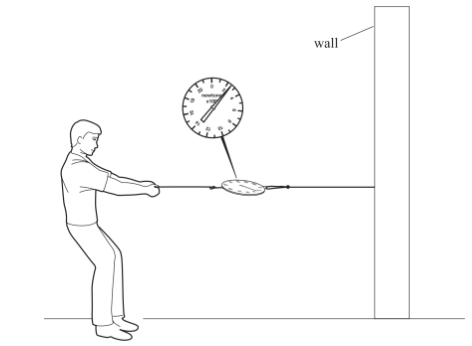
\includegraphics[width=6cm]{physics/figures/figure-unit-2-student.png}
\end{center}

Which statement correctly describes the amount of force applied by the wall on the student as they apply a \SI{250}{N} force?
    
\begin{randomizechoices}[norandomize]
    \choice The wall applies a force of 125 N against the student.
    \correctchoice The wall applies a force of 250 N against the student.
    \choice The wall applies twice as much force as the student.
    \choice The wall applies no force since it is stationary.
\end{randomizechoices}

\question 
When a bug hits the windshield of a car traveling at \SI{40}{mph}, the force of the bug on the windshield is

\begin{randomizechoices}[norandomize]
    \choice Greater than the force of the windshield on the bug.
    \choice Less than the force of the windshield on the bug.
    \correctchoice The same as the force of the windshield on the bug.
\end{randomizechoices}

\question
A student measuring the velocity and time of a toy car wrote down the following data.

\begin{center}
    \begin{tabular}{|c|c|c|c|c|c|c|}
        \hline
        \textbf{Velocity} (m/s) & \SI{4}{m/s} &  \SI{4}{m/s} & \SI{2}{m/s} & \SI{2}{m/s} & \SI{2}{m/s} & \SI{2}{m/s} \\ \hline
        \textbf{Time} (s) & \SI{0}{s} & \SI{2}{s} & \SI{4}{s} & \SI{6}{s} & \SI{8}{s} & \SI{10}{s} \\
        \hline
    \end{tabular}
\end{center}

What happened during the time interval between 2--4 seconds?

\begin{randomizechoices}[norandomize]
    \choice An unbalanced force was applied to the car increasing the car’s velocity.
    \correctchoice An unbalanced force was applied to the car, decreasing the car’s velocity.
    \choice A balanced force was applied to the car increasing the car’s velocity.
    \choice A balanced force was applied to the car, decreasing the car’s velocity.   
\end{randomizechoices}


\question 
Given the following image of a person on a bicycle, which of the following statements is correct about the cyclist’s motion?


\begin{center}
    \begin{tikzpicture}
        \node at (0,0) {\reflectbox{\twemoji[height=2cm]{man biking}}};
        \draw[thick,<-,right=1.5cm] (0,0) -- (1,0) node[above,pos=0.5] {5\,N};
        \draw[thick,<-,left=1.5cm] (0,0) -- (-1,0) node[above,pos=0.5] {5\,N};
        \draw[thick,<-,above=1.2cm] (0,0) -- (0,2) node[right,pos=0.5] {20\,N};
        \draw[thick,<-,below=1.2cm] (0,0) -- (0,-2) node[right,pos=0.5] {20\,N};
    \end{tikzpicture}
\end{center}

\begin{randomizechoices}
    \choice The person’s kinetic energy is changing with respect to time.
    \choice The person’s velocity is changing with respect to time.
    \correctchoice The person’s position is changing with respect to time.
    \choice The person’s momentum is changing with respect to time.
\end{randomizechoices}

\question 
Which of the following graphs represents an object with no momentum?

\begin{center}
    \begin{tikzpicture}
        \draw[->] (0,0) -- (0,2.5) node[above,rotate=90,pos=0.5] {Velocity (m/s)};
        \draw[->] (0,0) -- (2.5,0) node[below,pos=0.5] {Time (s)};
        \draw[ultra thick] (0,1.5) -- ++(2,0);
        \node at (1.25,2.8) {\textbf{Graph A}};
    \end{tikzpicture}
    \hspace{2em}
    \begin{tikzpicture}
        \draw[->] (0,0) -- (0,2.5) node[above,rotate=90,pos=0.5] {Velocity (m/s)};
        \draw[->] (0,0) -- (2.5,0) node[below,pos=0.5] {Time (s)};
        \draw[ultra thick] (0,0) -- (2,2);
        \node at (1.25,2.8) {\textbf{Graph B}};
    \end{tikzpicture}
    \hspace{2em}
    \begin{tikzpicture}
        \draw[->] (0,0) -- (0,2.5) node[above,rotate=90,pos=0.5] {Position (m)};
        \draw[->] (0,0) -- (2.5,0) node[below,pos=0.5] {Time (s)};
        \draw[ultra thick] (0,1.5) -- ++(2,0);
        \node at (1.25,2.8) {\textbf{Graph C}};
    \end{tikzpicture}
    \hspace{2em}
    \begin{tikzpicture}
        \draw[->] (0,0) -- (0,2.5) node[above,rotate=90,pos=0.5] {Position (m)};
        \draw[->] (0,0) -- (2.5,0) node[below,pos=0.5] {Time (s)};
        \draw[ultra thick] (0,2) -- (2,0);
        \node at (1.25,2.8) {\textbf{Graph D}};
    \end{tikzpicture}
\end{center}

\begin{randomizeoneparchoices}[norandomize]
    \choice Graph A
    \choice Graph B
    \correctchoice Graph C
    \choice Graph D
\end{randomizeoneparchoices}

% \question
% The following is a kinetic energy vs time graph made by a student doing a lab.  

% \begin{center}
%     \begin{tikzpicture}
%         \draw[->] (0,0) -- (0,3) node[above,pos=0.5,rotate=90] {Kinetic Energy};
%         \draw[->] (0,0) -- (3,0) node[below,pos=0.5] {Time};
%         \draw[ultra thick,domain=0:2.8] plot (\x,0.3*\x^2);
%     \end{tikzpicture}
% \end{center}

% Which of the following descriptions best represents what is happening to the object.

% \begin{randomizechoices}[norandomize]
%     \choice The forces are balanced and the kinetic energy is increasing.
%     \choice The forces are balanced and the kinetic energy is constant.
%     \choice he forces are unbalanced and the kinetic energy is constant.
%     \correctchoice The forces are unbalanced and the kinetic energy is changing.
% \end{randomizechoices}

\question 
When all individual forces acting on an object are balanced, it is the natural tendency of an object to 

\begin{randomizechoices}[norandomize]
    \choice eventually stop
    \choice accelerate
    \choice either speed up or slow down
    \correctchoice keep its velocity constant (either at a zero or non-zero value)
\end{randomizechoices}

\question 
A car is moving to the right as shown in the following motion map. 

\begin{center}
    \begin{tikzpicture}
        \begin{axis}[width=12cm,height=2.5cm,
            axis lines=none,
            xmin=0,xmax=1,
            ymin=0,ymax=1,
            clip=false,
            ]
            \draw[domain=0:1,samples=10,only marks,mark=*] plot({\x^0.5},0);
            \draw[<-,thick] (0,0.2) -- ++(0,0.8) node[above] {Start};
            \draw[<-,thick] (1,0.2) -- ++(0,0.8) node[above] {Finish};
        \end{axis}
    \end{tikzpicture}
\end{center}

Which of the following statements best represents the car’s motion?

\begin{randomizechoices}[norandomize]
    \choice The forces on the car are balanced and the car’s momentum is changing.			
    \choice The forces on the car are unbalanced and the car’s momentum is constant.
    \choice The forces on the car are balanced and the car’s momentum is constant.
    \correctchoice The forces on the car are unbalanced and the car’s momentum is changing.
\end{randomizechoices}

\question
Given this car towing a trailer, what can you say about its motion?

\begin{center}
    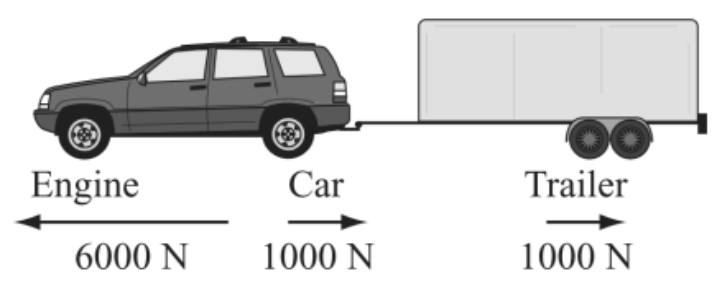
\includegraphics[width=6cm]{physics/figures/figure-unit-2-trailer.png}
\end{center}

\begin{randomizechoices}[norandomize]
    \choice The car’s forces are balanced so it is not moving or moving with a constant velocity.
    \choice The car’s forces are balanced so it has an overall change in its velocity.
    \choice The car’s forces are unbalanced and it is moving with a constant velocity.
    \correctchoice The car’s forces are unbalanced so it has an overall change in its velocity.    
\end{randomizechoices}


\ifversionKlevel
\begin{EnvUplevel}
    \textbf{Questions \ref{71tbo}--\ref{3M4Xb}.} The free-body diagram below represents an object moving to the right.
\end{EnvUplevel}


\begin{center}
    \begin{tikzpicture}
        \fill (0,0) circle (5pt);
        \draw[ultra thick,<->] (0,-1) -- (0,1);
        \draw[ultra thick,<->] (-2,0) -- (1,0);
    \end{tikzpicture}
\end{center}

\question \label{71tbo}
The object is\dots .

\begin{randomizechoices}[norandomize,keeplast]
    \choice speeding up
    \correctchoice slowing down
    \choice moving at constant speed 
    \choice none of the above
\end{randomizechoices}

\question \label{3M4Xb}
Are the force on the object balanced or unbalanced?

\begin{randomizeoneparchoices}[norandomize]
    \choice balanced
    \correctchoice unbalanced
\end{randomizeoneparchoices}

\fi

\clearpage

\ifprintanswers
    \printkeytable
\fi

\clearpage

\question[3]
Draw the free-body diagram of an open laptop that is resting on a table. Include all forces on the laptop and label them correctly. 

% \begin{parts}
%     \part[1] Correctly represent the laptop in the free-body diagram.
%     \part[1] Draw all the forces on the laptop.
%     \part[1] Label each force with a symbol and the type of force.
% \end{parts}

\begin{solutionorbox}[6cm]
\begin{center}
\begin{tikzpicture}
    \fill (0,0) circle (5pt);
    \draw[->,thick] (0,0) -- (0,-2) node[below,align=center] {$F_g$\\force of gravity};
    \draw[->,thick] (0,0) -- (0,+2) node[above,align=center] {normal force\\$F_N$};
\end{tikzpicture}
\end{center}
\end{solutionorbox}


\question[3]
A truck momentarily skids eastward along an bridge. Assume the frictional force between the truck and bridge is zero. Draw a force schema of the three interacting objects, identifying all force pairs. 

\begin{solutionorbox}[10cm]
(a) The three interaction objects: the truck, the bridge, the earth.

(b), (c)

\begin{center}
\begin{tikzpicture}
    \coordinate (earth) at (0,0); 
    \coordinate (bridge) at ({4},0); 
    \coordinate (truck) at ({4*cos(60)},{4*sin(60)}); 
    \draw (truck) node[above] {truck};
    \draw (bridge) node[right] {bridge};
    \draw (earth) node[left] {earth};
    \draw[ultra thick,<->] (truck)  -- (bridge) node[right=3pt,pos=0.1] {$F_\text{truck-bridge}$} node[right=3pt,pos=0.8] {$F_\text{bridge-truck}$};
    \draw[ultra thick,<->] (truck) -- (earth) node[left=3pt,pos=0.1] {$F_\text{truck-earth}$} node[left=3pt,pos=0.8] {$F_\text{earth-truck}$};
    \draw[ultra thick,<->] (earth) -- (bridge) node[below=3pt,pos=0.2] {$F_\text{earth-bridge}$} node[below=3pt] {$F_\text{bridge-earth}$};
\end{tikzpicture}
\end{center}    
\end{solutionorbox}

\clearpage
\question[5]
For each scenario, identify the type of force involved. Write your answer in the space provided.

\begin{enumerate} %...These scenarios were generated by ChatGPT.
    \item A climber dangles from a rope, feeling the strain as the ground seems miles away. What type of force does the rope exert? \\[1ex]
    \fillin[tension force][5cm]
    \item An apple falls from a tree, accelerating as it heads toward the earth. \\[1ex]
    \fillin[gravity][5cm]
    \item A book rests peacefully on a table, perfectly balanced, resisting the pull downward. What type of force does the table exert? \\[1ex]
    \fillin[normal force][5cm]
    \item Superman pushes a car down the road. \\[1ex]
    \fillin[applied force][5cm]
    \item A skateboarder grinds to a halt, shoes scraping the pavement as momentum fades.\\[1ex]
    \fillin[friction force][5cm]
\end{enumerate}

% \begin{solutionorlines}[7cm]
% \phantom{.}

% \begin{enumerate}
%     \item Tension force. Tension is a force that acts along a connecting medium, in this case the rope.
%     \item Gravitational force. Gravity is the force that pulls things downward towards the Earth.
%     \item Normal force. The normal force is applied by the table in the upward direction to support the book's weight.
%     \item Applied force. One car makes contact and pushes the other car.
%     \item Friction force. Friction arises when the shoes make contact with the ground and opposes the skater's direction.
% \end{enumerate}
% \end{solutionorlines}


\question
A car is driving down a straight road. Its motion map is shown below.

\begin{center}
    \begin{tikzpicture}[scale=0.7]
        \draw[domain=-10:0,mark=*,only marks, samples=6,mark size=3pt] plot({0.1*\x^2},0);
        \node at (-11.5,0.3) {\reflectbox{\twemoji[width=8mm]{automobile}}};
        \draw[thick,->] (-12,0.8) -- ++(1,0) node[above,pos=0.5] {$v$};
    \end{tikzpicture}
\end{center}

\begin{parts}
    \part[1] Is the car speeding up, slowing down, or moving at a constant speed?
    \part[1] Are the forces on the car balanced or unbalanced?
    \part[2] Draw one of the Multiple Representations of the object's motion.
\end{parts}

\begin{solutionorbox}[7cm]
(a) The car is slowing down, since the spacing between the dots is decreasing.

(b) The forces are unbalanced, since the object's velocity is changing. 

(c) Any one of the representations below:

\begin{center}
    \begin{tikzpicture}
        \begin{axis}[height=4cm,
            width=4cm,
            ymin=0,ymax=7,
            xmin=0,xmax=3,
            ticks=none,
            axis lines=left,
            ylabel={Position},
            xlabel={Time},
        ]
            \addplot[domain=0:2.5,ultra thick,black] {5*x - (100/(2*50))*x^2};
        \end{axis}
    \end{tikzpicture}
    \hspace{1em}
    \begin{tikzpicture}
        \begin{axis}[height=4cm,
            width=4cm,
            ymin=0,ymax=6,
            xmin=0,xmax=3,
            ticks=none,
            axis lines=left,
            ylabel={Velocity},
            xlabel={Time},
        ]
            \addplot[domain=0:2.5,ultra thick,black] {5 - 100/50*x};
        \end{axis}
    \end{tikzpicture}
    \hspace{1em}
    \begin{tikzpicture}
        \begin{axis}[height=4cm,
            width=4cm,
            ymin=0,ymax=300,
            xmin=0,xmax=3,
            ticks=none,
            axis lines=left,
            ylabel={Momentum},
            xlabel={Time},
        ]
            \addplot[domain=0:2.5,ultra thick,black] {50*5 - 100*x};
        \end{axis}
    \end{tikzpicture}
    \hspace{1em}
    \begin{tikzpicture}
        \begin{axis}[height=4cm,
            width=4cm,
            ymin=0,ymax=700,
            xmin=0,xmax=3,
            ticks=none,
            axis lines=left,
            ylabel={Kinetic Energy},
            xlabel={Time},
        ]
            \addplot[domain=0:2.5,ultra thick,black] {0.5*50*(5 - 100*x/50)^2};
        \end{axis}
    \end{tikzpicture}

    \bigskip

    \begin{tikzpicture}
        \draw[->] (0,-1) -- (0,1) node[above,rotate=90,pos=0.5] {Net Force};
        \draw[->] (0,0) -- ++(2,0) node[right,] {Time};
        \draw[ultra thick] (0,-0.5) -- ++(1.7,0);
    \end{tikzpicture}
\end{center}

\end{solutionorbox}

\end{questions}
\end{document}

